

\section{Introduction}
\label{sec:intro}
\begin{figure}[t]
 \centering
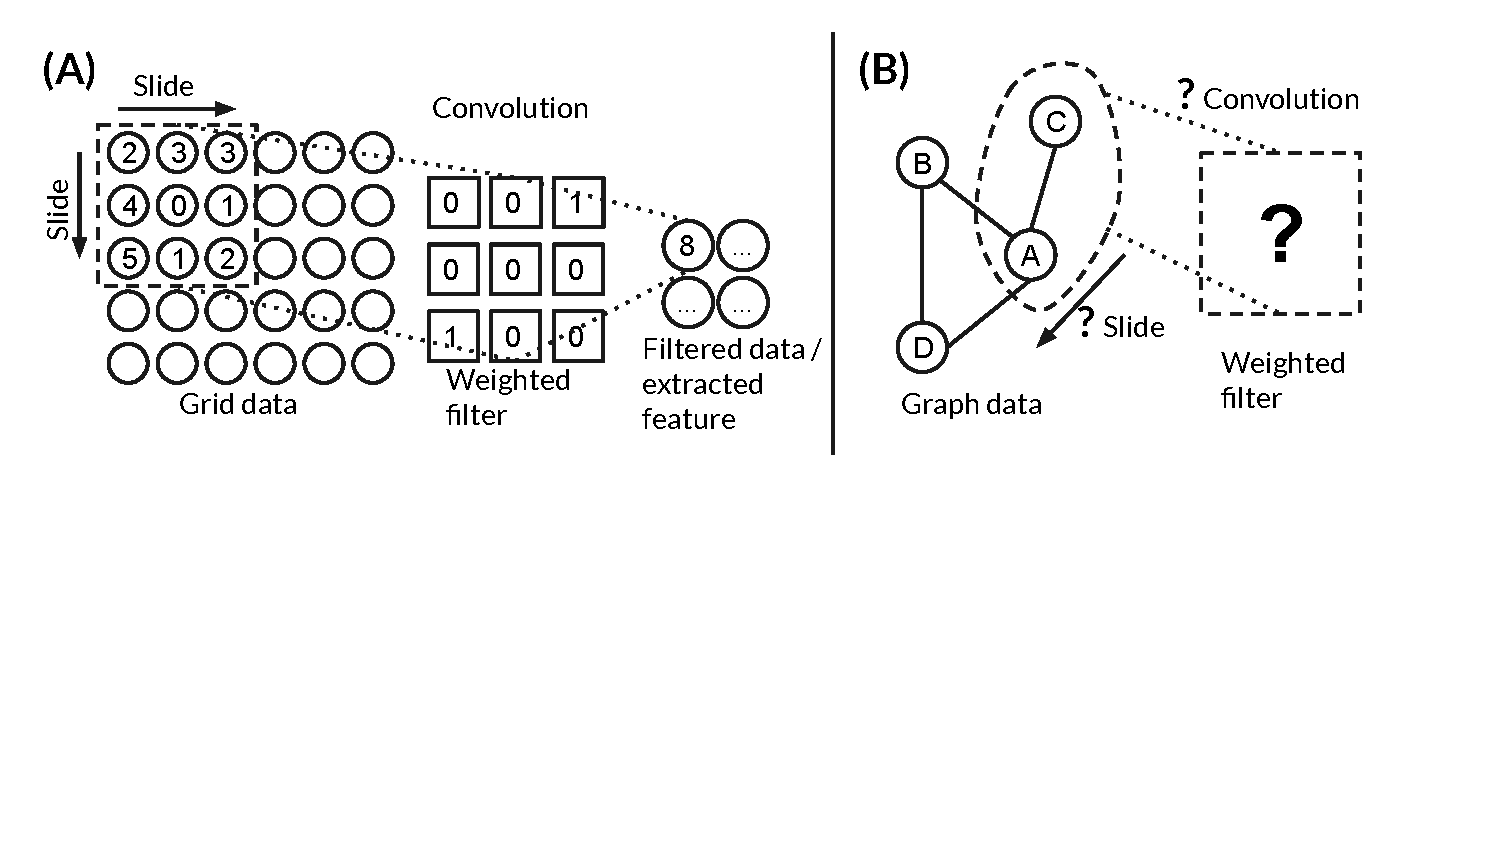
\includegraphics[width=0.49\textwidth]{./images/gridvsgraph.pdf}
 \caption{(A): Illustration of convolution on grid data such as image. (B): Natural operations such as translation and convolution on grid are non-trivial to define on graph data.}
 \label{fig:gridvsgraph}
\end{figure}

Deep neural networks, or deep learning, have revolutionized many domains like machine translation, computer vision, and natural language processing. They have proven to be highly effective in extracting complex and implicit features from the data. In many classical applications, the data is naturally represented as regular grids, such as images with their RGB pixel values. Techniques such as CNN~\cite{cnn0, cnn1, cnn2} are effective in capturing the local and shift-invariant information within an image. 

However, not all data has a simple grid or sequence shape; many data are naturally represented as graphs, while many other data can also be transformed into graphs~\cite{Xu2017}. Examples of graph data range from social and citation network~\cite{social, citation}, protein-protein interaction~\cite{ppi}, to point clouds~\cite{pointcloud}. Unfortunately, applying classical deep learning methods on graph data is not trivial, as graph data can have a rather irregular topology, and each node may have a different number of neighbors. There may not be ordering among the neighbors. Furthermore, the neighbors could be very distinct from each other, and there can also be information associated with the edges. These characteristics would make deep learning primitives such as convolution hard to define. As Figure~\ref{fig:gridvsgraph} presents, natural operations such as translation and convolution on a grid are not trivial to define for graph data.

Apart from the structural complexity, another distinctive characteristic of graphs is the absence of the i.i.d. assumption. In a classical machine learning setting, data points are usually assumed to be independently sampled from their actual distribution. However, data embedded in a graph as nodes are often explicitly connected, and these data are inherently non-i.i.d. This has complex implications when it comes to sub-sampling of graph data.

As such, there have been two directions to bring deep learning to graph data. The first route is by converting the graph data into the regular form to utilize existing deep learning methods; a prominent example is ~\cite{deepwalk}. The second route is developing new deep learning techniques or repurposing old techniques to work on graph data; these newly proposed techniques are known as Graph Neural Networks (GNN). This field has gained lots of attention recently and is the main topic of this paper.

Past efforts on GNNs can be roughly categorized into three divisions: the recurrent GNNs, spatial-based convolutional GNNs, and spectral-based convolutional GNNs~\cite{compsurvey}. The recurrent GNN and spatial-based convolutional GNN share very much in common, and they both explicitly leverage the structure and spatial localities of graphs. Hence, in some literature, they are also called spatial methods, while spectral-based convolutional GNNs are called spectral methods. Unlike spatial methods derived from deep learning research, spectral methods have a rather different lineage as they rise from the graph signal processing community. We will dive into the details later.
%
%GNNs have been used for various tasks, from local feature learning of node/edge embedding to global feature learning of graph embedding. They also have applications ranging from node classification, edge prediction, to generative tasks. These techniques have been used in various domains such as drug discovery~\cite{drugdis}, transportation research~\cite{trans}, particle physics~\cite{hep}, and many more domains~\cite{ss}

GNN research has not been solely focused on improving the accuracy performance of benchmark datasets. Lots of works focus on the system issues such as memory footprint and scalability~\cite{graphsage, fastgcn}. Apart from the algorithmic research and various techniques to bring down the computational cost, GNNs have also received attention from the system community. Just as the classical deep learning techniques need to be repurposed for GNNs, the underlying systems used for training/inference also need to change. The majority of the deep learning systems~\cite{tf, torch} had very little design consideration for graph data. As a result, their interfaces are unnatural for programming GNNs~\cite{dgl}, and their runtime performance is not optimal. 

Recently a new branch of system research has emerged: GNN systems~\cite{dgl}. These systems mainly focus on GNN model training and inference and optimize the execution to save time and avoid OOM errors. They are specifically tailored for graph data and GNN workloads, and they often offer orders of magnitude acceleration~\cite{dgl, pyg} over the classical deep learning systems.

Many surveys on GNNs exist~\cite{compsurvey, yannsurvey, zhousurvey} in the literature. However, none of them emphasizes the system issues and includes the newest advances in the GNN system domain. This paper is a short survey of GNN focusing on research related to the system issues of GNN. In addition to the algorithmic advancements, this paper will also go over some of the state-of-arts of GNN systems and provide potential future research directions. 

This paper is organized as follows: Section~\ref{sec:background} goes over some necessary backgrounds. Section~\ref{sec:gnn} covers various GNN architectures and the system issues and trade-offs associated with them. Section~\ref{sec:gnnsys} briefly introduces the emerging research field of GNN systems. Finally, Section~\ref{sec:conclusion} concludes this survey and discusses future research directions. 

%----------------------------------------------


\vspace{-2mm}
\section{Background and Preliminaries}
\label{sec:background}
\subsection{Deep Neural Networks}
Deep neural networks, or deep learning, have revolutionized many domains. To summarize its capability: one writes a set of simple goals (loss functions). Then, the program can automatically learn a way to represent the data and generate predictions for new data. Some prominent examples include CNNs~\cite{cnn2} and RNNs~\cite{rnn}. 

Recently other architectures such as Generative Adversarial Networks (GANs)~\cite{gan} and pure attention mechanism-based methods such as Transformers~\cite{transformer} have also greatly shaped the landscape. 

However, these techniques were majorly developed for regular-shaped data, such as tabular data, images, and time series. Naively applying deep learning to graph data is not viable. The model now needs to consider the underlying topology of the graph and must be capable of following the data relationship defined in the graph; the i.i.d. assumption commonly found in a lot of datasets may not hold for graph data. Therefore, graph data requires special treatment, and the DNN techniques usually need to be tweaked before applying to graph data.
%\subsection{Graph Analytics and Tasks}
%Graph analytics is a topic that has much longer history than GNNs. There have been abundant research and attempts to reason about graph data and extract valuable information from them. GNNs are among the newest additions to the arsenal of graph analytics and they have gained lots of attention. GNN, as  
%Node classification. Edge prediction. Graph embedding.
%
%\subsection{History of Graph Neural Networks}
%Prior to GNNs, there have been abundant research on graph analytics. However, the commonly acknowledged first published work on GNN was~\cite{gnn0}. This work purposed the first Recurrent GNN to better distinguish


\subsection{Machine Learning Systems for Efficient Model Training and Inference}
%The success of DNNs does not solely come from algorithmic advancements but is a combination of revolutions in computational hardwares~\cite{cuda}, availability of unprecedented large datasets (Big Data)~\cite{imagenet, coco}, and efficient and scalable systems designed for these novel workloads~\cite{tf, spark}. 
Because of the booming of DNN and their massive adoption across academia and industry, the demand for reliable, easy-to-use, and efficient software also skyrocketed~\cite{tf, torch, spark}. There are many aspects of the machine learning life cycle, from data sourcing, cleaning to model training and inference. Among these topics, model training and inference are arguably among the ones that face the most scalability and efficiency challenges; the complexity of the models and the amount of data has been rapidly growing up~\cite{gpt-3, toi}. It is vital for the model training and inference systems to keep up with the pace to enable such workloads at scale.  Again, due to the unique nature of graphs and GNNs, existing systems need to be tweaked and specialized for GNN workloads.

\subsection{Notations and Definitions}
We now summarize the set of notations and definitions used throughout the paper. Table~\ref{tab:notation} presents all the notations. We now give the definitions of several concepts. 
\begin{enumerate}
\item \textbf{Graph.} A graph $G(V, E)$ is defined as a collection of nodes $V$ and edges $E$ connecting the nodes. The graph can be directed or undirected, cyclic or acyclic. 
\item \textbf{Node and edge features.} Each node $v \in V$ can have a $D_v$-dimensional node feature vector $\mathbf{x}_v \in \mathbb{R}^{D_v}$. Similarly, each edge $e \in E$ can also have a $D_e$-dimensional edge feature $\mathbf{x}_e \in \mathbb{R}^{D_n}$. Stack these features as column-vectors to form matrix, we have matrix $\mathbf{X}_n \in \mathbb{R}^{D_v \times |V| }$ and $\mathbf{X}_e \in \mathbb{R}^{D_e \times |E|}$.
\item \textbf{Weights and model parameters.} Throughout the paper, the learnable weights of neural networks are typically denoted as $w$ (scalar), $\mathbf{w}$ (vector), or $\mathbf{W}$ (matrix). When it comes to weight matrices composed of weight vectors, they are usually row-based, in contrast to feature vectors and matrices. 
\item \textbf{Node neighbors.} Given a node $v$, the function $\mathcal {N}$ returns the set of all 1-hop neighbors of $v$, including the node itself. Similarly, define $\hat {\mathcal {N}}$ to be the function that returns all neighbors of a node, excluding itself. This includes both the nodes with edges pointing to $v$, and nodes pointed by $v$.
\item \textbf{Node embeddings and hidden states.} Node embeddings are representations of nodes in a Euclidean space through a usually learned mapping. They contain information about the node. In this paper, we use hidden states and node embeddings interchangeably. We use $\mathbf{h_v}$ throughout the paper to denote the node embeddings. The dimensionality $D_h$ is determined by the graph neural network and is usually a hyperparameter.
\item \textbf{Graph Laplacian.} Graph Laplacian is a matrix representation of the graph. It is very important in spectral graph theory and spectral-based convolutional GNNs, please refer to Section~\ref{sec:spectral} for details.
\end{enumerate}



